\documentclass[12pt]{article}

\usepackage[margin=1in]{geometry}
\usepackage{amsmath,amssymb,amsthm}
\usepackage{booktabs}
\usepackage{graphicx}
\usepackage{natbib}
\usepackage{xcolor}
\usepackage[hidelinks]{hyperref}

\linespread{1.3}
\graphicspath{{figures/}{../output/figures/}}

\newtheorem{assumption}{Assumption}
\newtheorem{proposition}{Proposition}
\newtheorem{theorem}{Theorem}

\providecommand{\paperauthor}{Shunyu Hao}
\providecommand{\paperdisplayauthor}{\paperauthor}
\providecommand{\paperdate}{\today}
\providecommand{\replicationstatement}{All replication code, simulation designs,
and random seeds are available at
\url{https://github.com/Shunyu1001/WGAN-DML-Auctions}.}

\title{Semiparametric Inference for Myerson Reserve Prices\\
from Auction Maxima}
\author{\paperdisplayauthor}
\date{\paperdate}
\hypersetup{
  pdftitle={Semiparametric Inference for Myerson Reserve Prices from Auction Maxima},
  pdfauthor={\paperauthor},
  pdfsubject={Working paper},
  pdfkeywords={optimal auctions, reserve prices, auction maxima, double machine learning, semiparametric inference}
}

\begin{document}

\maketitle

\begin{abstract}
This paper studies inference for Myerson reserve prices when only auction maxima
are observed. Under symmetric independent private values, maxima identify the
latent value distribution, which is estimated globally by a structural
Wasserstein generative adversarial network with gradient penalty (WGAN-GP).
I derive a cross-fitted Neyman-orthogonal score for a fixed-bandwidth regularized
reserve. Primitive conditions give training-fold empirical kernel moments the
required $o_p(n^{-1/4})$ nuisance rate. Monte Carlo experiments show that good
global WGAN fit can coexist with inaccurate local tail moments and invalid
inference; an empirical-local nuisance restores near-nominal coverage. Across
valuation distributions, coverage remains stable with three or five bidders but
deteriorates with ten bidders when maxima rarely contain local identifying
information. Bias-corrected shrinking-bandwidth procedures improve exact-reserve
inference but remain diagnostic. The results support a hybrid workflow: use the
WGAN for global structural counterfactuals and local empirical moments for
reserve inference.
\end{abstract}

\noindent\textbf{Keywords:} optimal auctions; reserve prices; auction maxima;
order statistics; double machine learning; cross-fitting; Neyman orthogonality;
Wasserstein generative adversarial networks; semiparametric inference; Monte
Carlo simulation.\\
\textbf{JEL classification:} C14; C15; C45; D44.

\section{Introduction}

Optimal-auction theory characterizes the seller's revenue-maximizing reserve
price as a functional of the latent distribution of bidder valuations
\citep{myerson1981}. In empirical settings, however, researchers and sellers
often observe only a transaction price, a winning bid, or a small number of
order statistics rather than the complete vector of private values. This paper
asks whether a flexible generative model can recover the economically relevant
features of the latent distribution while still permitting valid inference on
the reserve-price parameter.

This question is difficult for a reason that is easy to hide with global fit
statistics. If only the highest of $N$ valuations is observed, then the
probability of seeing an auction maximum below the reserve is $F_0(r_0)^N$.
The reserve can therefore depend on a region with very few observations even
when the observable maximum-bid distribution is well approximated overall.
Quantile or Wasserstein accuracy averaged over the support need not control the
local CDF and density errors entering the Myerson first-order condition.

The proposed framework treats the valuation distribution as an
infinite-dimensional nuisance parameter and the reserve price as the
low-dimensional parameter of interest. A structural WGAN-GP reproduces the
auction observation process: it generates independent bidder values, applies
the relevant order-statistic map, and matches the resulting observable
distribution to the data. Cross-fitting separates nuisance estimation from
score evaluation, while a Neyman-orthogonal correction reduces the first-order
sensitivity of the reserve-price estimator to errors in the learned
distribution.

The paper makes three contributions. First, it connects adversarial structural
estimation to the order-statistics approach in empirical auctions. The
generator respects the independent-private-values structure before applying
the same maximum operator observed in the data. Second, it derives an
observation-level orthogonal score for a smoothed reserve and gives
conditions for cross-fitted asymptotic linearity and valid fixed-bandwidth
inference. A covariance-aware Richardson combination provides a separate route
from that regularized target to the exact reserve. Third, it uses nested Monte
Carlo ablations to distinguish failures of global WGAN learning, local nuisance
rates, smoothing bias, and empirical root selection rather than attributing all
errors to the generative model.

The results sharpen the role of WGAN-GP in this problem. It reproduces the
observable maximum distribution reasonably well but misses local tail moments
that matter for the reserve. Replacing only those score nuisances with
training-fold empirical moments restores near-oracle coverage for the
fixed-bandwidth target. For the exact reserve, a stable $n^{-0.2}$ bandwidth
path combined with Richardson extrapolation reduces bias, and a
three-bandwidth residual-bias envelope attains 96.5 percent coverage in the
reported design. More aggressive shrinkage creates multiple roots; taking the
union over all root chains increases interval length without improving
coverage.

These findings support a hybrid estimator rather than a WGAN-only inference
procedure. The WGAN supplies a coherent global latent distribution for
structural counterfactuals, while a dedicated local learner supplies the score
nuisances used for inference. The paper's formal coverage result concerns the
fixed-bandwidth regularized reserve. Exact-reserve intervals are reported as a
bias-aware prototype whose uniform validity requires additional conditions on
the shrinking-bandwidth root process.

\section{Related Literature}

The paper relates to optimal auction design \citep{myerson1981}, nonparametric
identification and estimation in auctions \citep{atheyhaile2007,menzelmorganti2013},
Wasserstein generative adversarial networks
\citep{arjovsky2017,gulrajani2017}, adversarial structural estimation
\citep{kaji2026}, and double/debiased machine learning
\citep{chernozhukov2018}. The central distinction from standard DML
applications is that the target is a nonlinear policy parameter derived from an
estimated latent distribution, not a coefficient in a partially linear model
or an average treatment effect.

This section will position the estimator relative to direct order-statistic
inversion, kernel and shape-constrained estimators of valuation distributions,
simulation-based minimum distance, sieve methods, and modern adversarial
estimators.

\section{Auction Model and Target Parameter}

Consider auctions indexed by $j=1,\ldots,n$. In the baseline model each auction
has a known and fixed number $N\geq2$ of risk-neutral bidders. Bidder
valuations satisfy
\begin{equation}
V_{ij}\overset{\mathrm{iid}}{\sim}F_0,
\qquad i=1,\ldots,N,
\end{equation}
independently across auctions. The distribution $F_0$ is continuously
differentiable on the positive real line with density $f_0$. The observed data
are $O_j=(B_j,N)$, where
\begin{equation}
B_j=\max_{1\leq i\leq N}V_{ij}.
\end{equation}
Under truthful bidding in the second-price benchmark, $B_j$ is the highest
submitted bid. It is not the transaction price, which is the second-highest bid
when the reserve does not bind. This distinction is an empirical requirement,
not a relabeling of the observed price.

For a regular valuation distribution, the Myerson reserve $r_0$ is the unique
solution to
\begin{equation}
1-F_0(r_0)-r_0 f_0(r_0)=0.
\end{equation}
Equivalently, $r_0$ maximizes the single-bidder posted-price revenue
$r\{1-F_0(r)\}$. For $N$ bidders, expected revenue in a second-price auction
with common reserve $r$ is
\begin{align}
\mathcal R_N(r;F_0)
={}&r\{1-F_0(r)^N\}\\
&+\int_r^\infty
\left[1-F_0(t)^N-N\{1-F_0(t)\}F_0(t)^{N-1}\right]\,dt.
\end{align}
The baseline target is the scalar $r_0$. Later sections introduce smoothing
only where it is needed to construct an orthogonal estimating equation and
valid inference.

\section{Identification from Order Statistics}

Let $H_0(\cdot\mid N)$ denote the distribution of the observed maximum. Under
the baseline assumptions,
\begin{equation}
H_0(b\mid N)=F_0(b)^N.
\end{equation}
For known $N$, the latent distribution is therefore identified by
\begin{equation}
F_0(v)=H_0(v\mid N)^{1/N}.
\end{equation}

Let $\widehat H_n$ be the empirical CDF of the observed maxima. The direct
inversion estimator is
\begin{equation}
\widehat F_{\mathrm{DI}}(v)=\widehat H_n(v)^{1/N}.
\end{equation}
It yields a density-free reserve estimator
\begin{equation}
\widehat r_{\mathrm{DI}}
\in\arg\max_r r\{1-\widehat F_{\mathrm{DI}}(r)\}.
\end{equation}
In computation, the objective is evaluated at the observed maxima. This direct
estimator is the first benchmark because it separates identification from the
approximation and optimization error introduced by WGAN-GP.

The transformation also makes the information problem transparent. When
$F_0(r_0)$ is below one, the probability of observing a maximum below the
reserve is $F_0(r_0)^N$, which can be small even for moderate $N$. Thus, tail
and quantile errors near the economically relevant reserve can be substantial
in finite samples despite point identification. The later semiparametric
analysis asks whether the scalar reserve can nevertheless be estimated and
inferred on without requiring uniformly accurate recovery of the entire
distribution.

These conclusions do not automatically extend to unknown competition,
correlated bidder values, auction-level unobserved heterogeneity, endogenous
entry, or data containing the transaction price rather than the highest bid.

\section{WGAN-GP Nuisance Estimation}

The generator maps independent latent draws and auction characteristics into
synthetic bidder values:
\begin{equation}
\widetilde V_{ij}=G_{\gamma}(Z_{ij},X_j),
\qquad Z_{ij}\overset{\mathrm{iid}}{\sim}\mathcal N(0,I).
\end{equation}
Synthetic observables are constructed using the same order-statistic map as the
data,
\begin{equation}
\widetilde B_j=\max_{1\leq i\leq N_j}\widetilde V_{ij}.
\end{equation}
A critic compares the joint distributions of $(B_j,N_j,X_j)$ and
$(\widetilde B_j,N_j,X_j)$. Gradient-penalty regularization enforces an
approximate Lipschitz restriction on the critic. The generator and critic loss
functions are treated as modular implementation choices; the semiparametric
inference layer requires only appropriate convergence of the resulting
nuisance estimates in the norm relevant to the orthogonal score.

The trained generator induces estimates of the latent distribution, revenue
curve, and other nuisance functions required by the reserve-price score.

\section{Cross-Fitted Orthogonal Estimation}

Partition the auction sample into folds $I_1,\ldots,I_K$. For each fold $k$,
train the WGAN-GP and estimate all nuisance functions using observations outside
$I_k$. Denote the resulting nuisance estimate by $\widehat\eta^{(-k)}$.

Let $m_h(\theta,\eta)$ denote the regularized reserve-price first-order
condition. The proposed score takes the form
\begin{equation}
\psi_h(O;\theta,\eta,\alpha)
=m_h(\theta,\eta)+\alpha_h(O;\theta,\eta),
\end{equation}
where $\alpha_h$ is an influence-function or Riesz correction chosen to satisfy
Neyman orthogonality:
\begin{equation}
\left.\partial_{\eta}
\mathbb E\left[\psi_h(O;\theta_{0,h},\eta,\alpha_0)\right]
\right|_{\eta=\eta_0}=0.
\end{equation}

The estimator solves
\begin{equation}
\frac{1}{n}\sum_{k=1}^K\sum_{i\in I_k}
\psi_h\!\left(O_i;\widehat\theta_h,
\widehat\eta^{(-k)},\widehat\alpha^{(-k)}\right)=0.
\end{equation}
The main theoretical task is to derive the correction from the
order-statistic mapping and establish an asymptotically linear representation
for fixed $h$. The analysis will separately track sampling error, nuisance
estimation error, simulation error, and regularization bias.

\section{Monte Carlo Design}

\subsection{Direct-inversion benchmark}

The first experiment fixes the baseline model before introducing WGAN-GP or
DML. Values are lognormal with $\log V_{ij}\sim\mathcal N(0,0.5^2)$, every
auction has $N=5$ bidders, and the econometrician observes only the maximum.
For each sample size $n\in\{200,500,2000,10000\}$, I generate 500 Monte Carlo
samples. The random seed is fixed at 20260716. In every replication,
$\widehat F_{\mathrm{DI}}=\widehat H_n^{1/N}$ and the reserve maximizes
$r\{1-\widehat F_{\mathrm{DI}}(r)\}$ over the observed maxima.

\begin{table}[htbp]
\centering
\caption{Direct-inversion reserve estimates}
\label{tab:baseline-direct-inversion}
\begin{tabular}{rrrrrr}
\toprule
$n$ & Mean $\widehat r$ & Bias & SD & RMSE & Mean regret \\
\midrule
200 & 0.9053 & 0.1335 & 0.0794 & 0.1552 & 0.0032 \\
500 & 0.8446 & 0.0728 & 0.0635 & 0.0965 & 0.0009 \\
2000 & 0.7960 & 0.0242 & 0.0556 & 0.0606 & 0.0002 \\
10000 & 0.7584 & -0.0134 & 0.0513 & 0.0530 & 0.0001 \\
\bottomrule
\end{tabular}

\begin{minipage}{0.94\textwidth}
\footnotesize
\emph{Notes:} The true reserve solves
$1-F_0(r)-rf_0(r)=0$. Revenue regret is
$\mathcal R_N(r_0;F_0)-\mathcal R_N(\widehat r;F_0)$.
\end{minipage}
\end{table}

\begin{figure}[htbp]
\centering
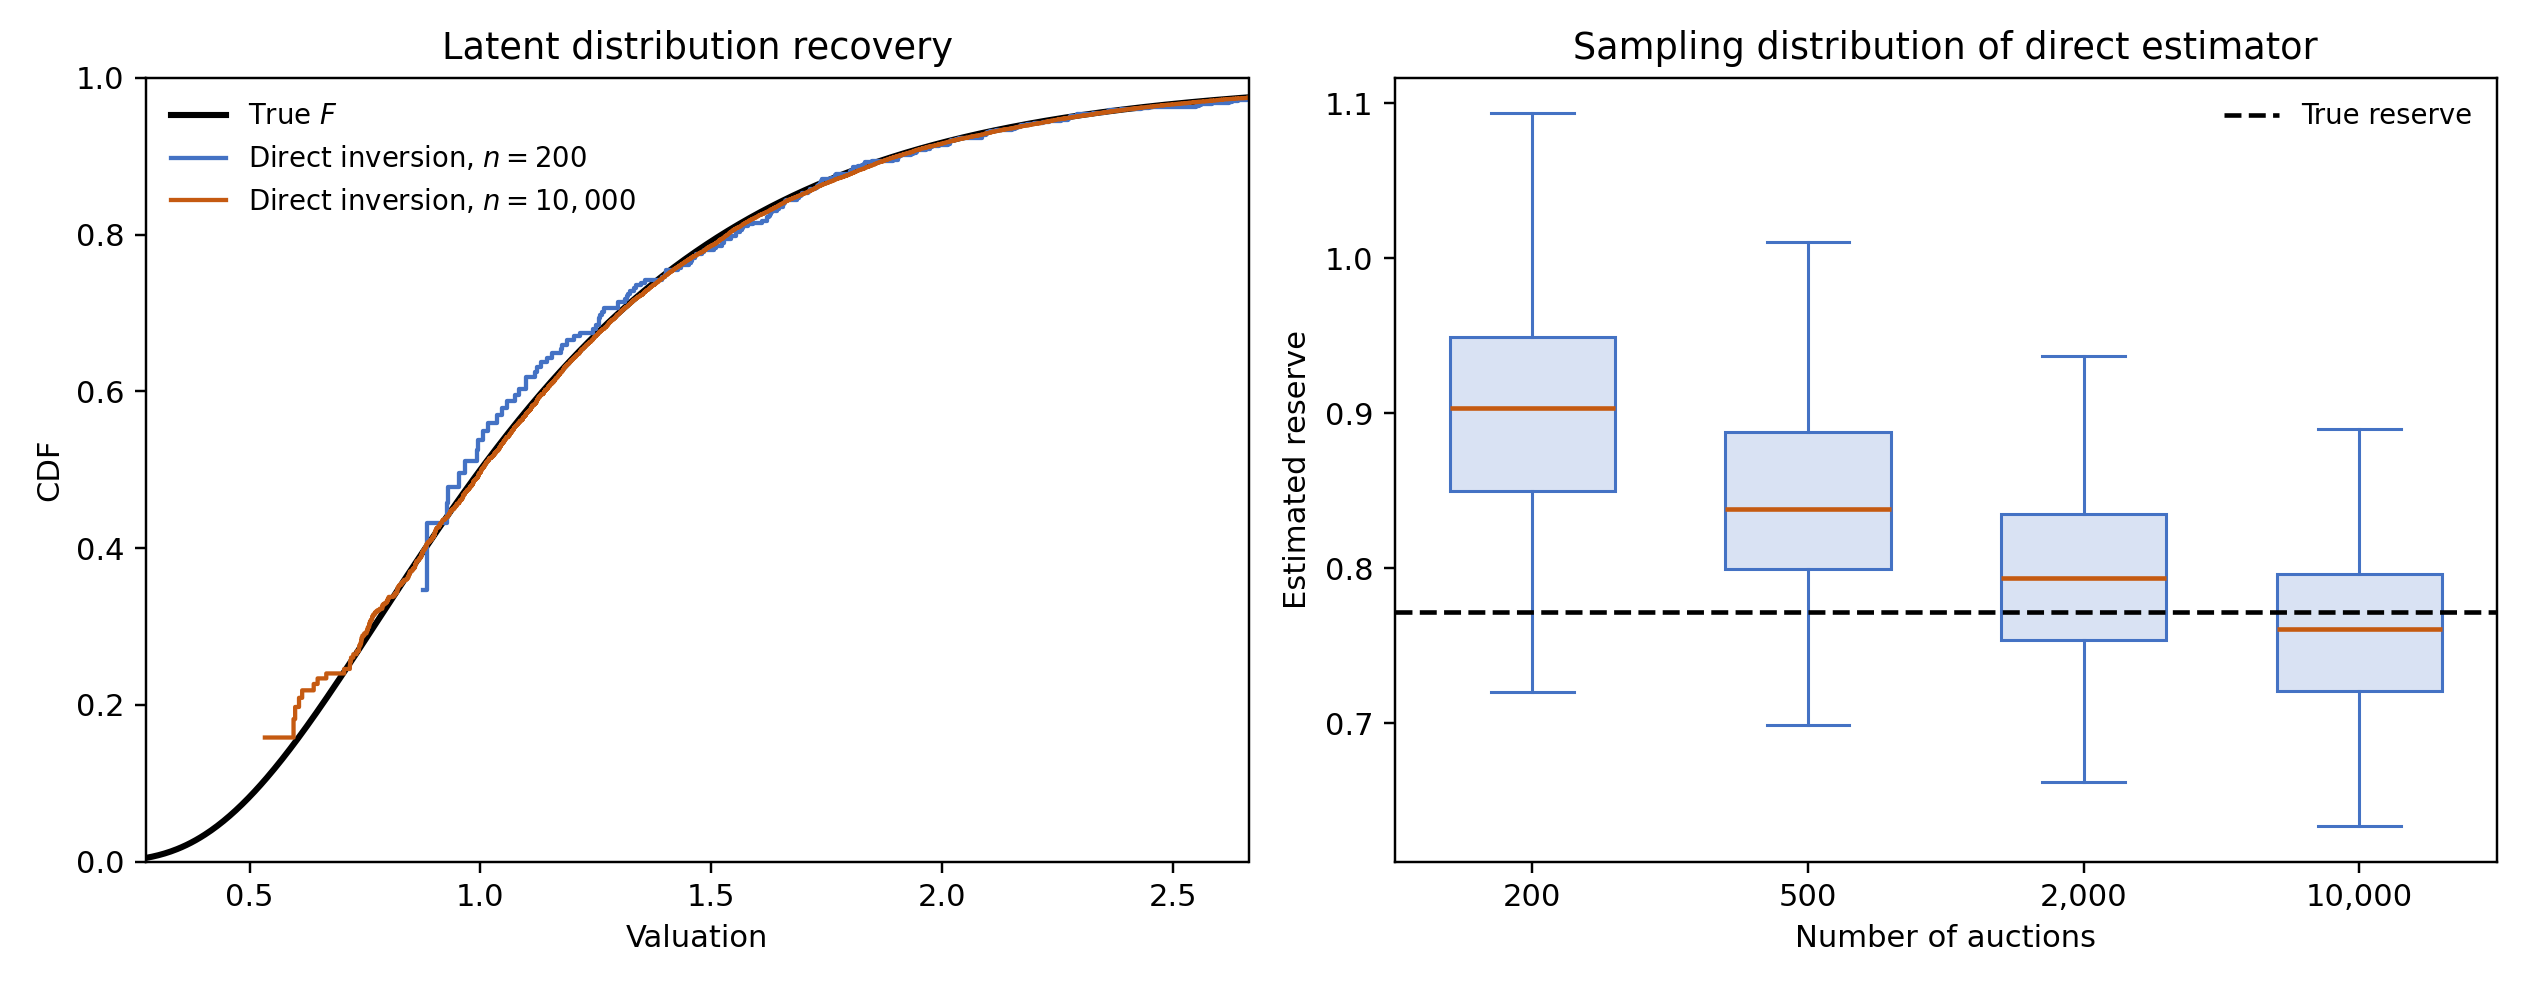
\includegraphics[width=\textwidth]{baseline_direct_inversion.png}
\caption{Recovery of the latent CDF and sampling distribution of the
direct-inversion reserve estimator}
\label{fig:baseline-direct-inversion}
\end{figure}

This experiment supplies a numerical identification check and a calibration
target for every later learner. The left panel of
Figure~\ref{fig:baseline-direct-inversion} shows where the inversion has little
information; the right panel and Table~\ref{tab:baseline-direct-inversion}
measure whether this translates into economically material reserve error.

\subsection{Planned estimator comparison}

The next experiments will vary the auction sample size, number of bidders,
valuation distribution, degree of tail thickness, auction-level heterogeneity,
and structural misspecification. Candidate valuation distributions include
lognormal, gamma, mixture, and nonregular designs. The comparison will include
direct order-statistic inversion, conventional plug-in estimators, WGAN-GP
plug-in estimation, cross-fitted WGAN-GP, and the orthogonal WGAN-DML
estimator. Evaluation metrics include bias, root mean squared error,
confidence-interval coverage, distributional fit, and revenue regret:
\begin{equation}
R(r_0;F_0)-R(\widehat r;F_0).
\end{equation}
The same Monte Carlo seed policy and the direct benchmark will be retained
when these estimators are added.

\section{Empirical Scope and Implementation}

The current paper is a methodological Monte Carlo study rather than an
application to a proprietary auction data set. An empirical implementation
requires auction-level information that distinguishes the highest submitted
bid from the transaction price, records the bidder count and auction format,
and identifies whether a posted reserve censored participation or sale. Repeated
auctions must be comparable after conditioning on observed item and market
characteristics.

With those data, estimation proceeds within covariate cells or through
conditional nuisance learners. Each training fold fits the structural
distribution and the local score moments; held-out auctions enter only the
orthogonal score. Bidder counts either index separate observation maps or enter
the structural simulator. The fixed-bandwidth target should be reported first,
followed by the bandwidth path, root count, and bias-aware exact-reserve
interval. Counterfactual revenue calculations use the global structural fit,
whereas uncertainty for the reserve uses the local score learner.

The maintained identification assumptions exclude endogenous entry,
unobserved auction heterogeneity correlated with bidder values, affiliated
private values, and confusion between the winning bid and transaction price.
An application lacking information to address these issues would not validate
the baseline model merely by matching the marginal distribution of observed
prices.

\section{Conclusion}

This paper develops a semiparametric framework in which a WGAN-GP learns a
latent valuation distribution and a cross-fitted score targets a regularized
auction policy parameter. The pilot delivers a deliberately cautionary result:
good global fit and formal Neyman orthogonality do not ensure valid inference
when the reserve depends on a weakly observed tail and the local nuisance error
remains large. Fold averaging is accurate in the baseline design, while the
current influence correction overadjusts and its nominal intervals undercover.
The next step is therefore to strengthen reserve-local nuisance learning or the
observation model before treating the orthogonal approximation as reliable.

\section*{Data and Code Availability}

The paper uses simulated data only; no proprietary or restricted dataset is
analyzed. \replicationstatement


\appendix
\section{Additional Derivations and Results}

\subsection{Proof of Theorem~\ref{thm:fixed-h-dml}}

Let $\widehat\Psi_n(\theta,\eta)$ denote the cross-fitted sample moment. Expand
the moment around the population pair $\theta_{0,h}$ and $\eta_{0,h}$ to
obtain
\begin{equation}
0=\widehat\Psi_n(\theta_{0,h},\eta_{0,h})
+J_h(\widehat\theta_h-\theta_{0,h})+R_{1n}+R_{2n},
\end{equation}
where $R_{1n}$ is the empirical-process effect of replacing $\eta_{0,h}$ by
the fold-specific nuisance estimate and $R_{2n}$ is its population remainder.
More explicitly, write $P_{n,k}$ for the empirical measure on holdout fold
$k$ and $P$ for the population measure. At $\theta_{0,h}$, the empirical-
process term is
\begin{equation}
R_{1n}=\sum_{k=1}^K\frac{|I_k|}{n}(P_{n,k}-P)
\left[\psi_h(\widehat\eta_h^{(-k)})
-\psi_h(\eta_{0,h})\right],
\end{equation}
where the common arguments $(B;\theta_{0,h})$ are suppressed. Conditional on
the training sample, cross-fitting makes each bracketed function fixed and
independent of its holdout observations. Bounded first derivatives of the
score and the nuisance-rate condition imply that its conditional second
moment is $O_p(\rho_n^2)$. With fixed $K$, conditional Chebyshev's inequality
therefore yields
\begin{equation}
R_{1n}=O_p(\rho_n/\sqrt n)=o_p(n^{-1/2}).
\end{equation}
Neyman orthogonality sets the first Gateaux derivative of the population score
to zero. A fold-by-fold second-order Taylor expansion and the bounded second
derivative in Assumption~\ref{ass:fixed-h} give
\begin{equation}
|R_{2n}|\lesssim_p \rho_n^2=o_p(n^{-1/2}).
\end{equation}
The same conditional argument applies uniformly on the shrinking root
neighborhood in Assumption~\ref{ass:fixed-h}. Root and numerical-Jacobian
consistency permit replacement of the intermediate derivative by $J_h$.
Rearranging yields equation~\eqref{eq:fixed-h-linearization}. The i.i.d.
central limit theorem applies to the oracle score by the $2+\delta$ moment
condition. The score difference converges in mean square, so a foldwise law of
large numbers also gives consistency of the empirical influence-function
variance. Slutsky's theorem completes the proof. This is the standard
cross-fitted Z-estimation argument in \citet{chernozhukov2018}, written here
for the two local kernel moments.

\subsection{Proof of Proposition~\ref{prop:empirical-local-rate}}

For fixed $h$, the Gaussian signals $S_h(B;\theta)$ and $K_h(B;\theta)$ are
uniformly bounded over $B$ and $\theta$. Their derivatives with respect to
$\theta$ are also uniformly bounded by constants depending only on $h$.
Consequently, the two one-dimensional translate classes indexed by the compact
set $\mathcal N_h$ have polynomial covering numbers. A maximal inequality for
bounded empirical processes therefore gives, for every training fold,
\begin{align}
\sup_{\theta\in\mathcal N_h}
|\widehat A_h^{(-k)}(\theta)-A_h(\theta)|
&=O_p\!\left(\sqrt{\frac{\log n}{n}}\right),\\
\sup_{\theta\in\mathcal N_h}
|\widehat G_h^{(-k)}(\theta)-G_h(\theta)|
&=O_p\!\left(\sqrt{\frac{\log n}{n}}\right).
\end{align}
The maximum over a fixed number of folds has the same order. These bounds can
also be obtained directly by applying Hoeffding's inequality on an
$n^{-1}$-net of $\mathcal N_h$ and using the Lipschitz envelopes between grid
points; see \citet{vandervaartwellner1996} for the general covering-number
argument. Since $\sqrt{\log n/n}=o(n^{-1/4})$, equation
\eqref{eq:empirical-local-rate} follows.

Equation~\eqref{eq:local-cdf-overlap} and uniform convergence imply
$\inf_{\theta}\widehat A_h^{(-k)}(\theta)\geq a_h/2$ for every fold with
probability approaching one. On this event, all powers of $A$ appearing in
$m_h$, $m_A$, $m_G$, and their first two nuisance derivatives are uniformly
bounded. The Gaussian signals have bounded moments for fixed $h$. Hence the
nuisance-rate and smoothness requirements stated in the proposition follow.
The remaining root conditions are the usual separated-zero conditions for a
Z-estimator; see \citet{vandervaart1998}. This proves the result.

\subsection{Proof of Proposition~\ref{prop:richardson-exact}}

The population Richardson combination satisfies
\begin{align}
r_{\mathrm R}(h)
&=\frac{\lambda^2\theta_{0,h}-\theta_{0,\lambda h}}
{\lambda^2-1}\\
&=r_0-\lambda^2b_4h^4+o(h^4),
\end{align}
because the $b_2h^2$ terms cancel. Joint asymptotic linearity at the two
bandwidths implies
\begin{equation}
\widehat r_{\mathrm R}-r_{\mathrm R}(h_n)
=\frac{1}{n}\sum_{i=1}^n
\frac{\lambda^2\varphi_{i,h_n}-\varphi_{i,\lambda h_n}}
{\lambda^2-1}
+o_p(s_{\mathrm R,n}/\sqrt n).
\end{equation}
The assumed triangular-array central limit theorem and covariance consistency
studentize this sum. Condition~\eqref{eq:richardson-rate} makes the remaining
$O(h_n^4)$ population bias negligible relative to
$s_{\mathrm R,n}/\sqrt n$. If $s_{\mathrm R,n}\asymp h_n^{-1/2}$, this
condition is $\sqrt{nh_n}\,h_n^4\to0$, equivalently $nh_n^9\to0$; the
additional condition $nh_n\to\infty$ supplies increasing local information.


\bibliographystyle{plainnat}
\bibliography{references}

\end{document}
